\section*{\underline{PART G: The Final Engineering Question}}
\markboth{PART G: The Final Engineering Question}{}

\subsection*{Question 20: What should the plant do to reduce machine downtime?}

To provide evidence-based recommendations to the plant manager, we must synthesize our statistical findings and translate them into actionable engineering directives. The primary objective is to reduce the overall mean repair time (currently at 16.36 minutes), compress the extreme variance (ranging from 3 to over 276 minutes), and mitigate the highest sources of cumulative downtime.

Based on our comprehensive analysis of the 635 recorded repair events (totaling 10,387.80 minutes of downtime), we have identified four critical areas for intervention.

\subsubsection*{1. Target the Mechanical Bottlenecks (Extruder Press \& Hacking Station)}

\textbf{Statistical Finding:} 
Downtime is not distributed evenly across the production line. A Pareto analysis of the stoppage locations reveals a severe concentration of failures at just two nodes: the Extruder Press and the Hacking Station. Together, they account for over 54\% of the plant's total downtime.

\begin{table}[H]
    \centering
    \resizebox{\textwidth}{!}{
    \begin{tabular}{lrrrr}
        \toprule
        \textbf{Stop Location} & \textbf{Repairs} & \textbf{Mean (min)} & \textbf{Total Downtime} & \textbf{Share (\%)} \\
        \midrule
        EXTRUDER PRESS & 169 & 18.00 & 3042.6 min & 29.29\% \\
        HACKING STATION & 181 & 14.20 & 2570.4 min & 24.74\% \\
        DRYER & 78 & 11.08 & 864.2 min & 8.32\% \\
        CUTTER & 64 & 11.60 & 742.3 min & 7.15\% \\
        HYD.\ ELEVATOR (UNLOADING) & 31 & 17.76 & 550.6 min & 5.30\% \\
        \bottomrule
    \end{tabular}
    }
    \caption{Top 5 Locations by Total Downtime Contribution}
    \label{tab:top_locations}
\end{table}

\textbf{Engineering Recommendation:}
Because this is a serial production line, a bottleneck at the Extruder Press halts the entire factory throughput. Maintenance leadership must prioritize these two stations. 
\begin{itemize}
    \item \textbf{Resource Colocation:} Position dedicated maintenance toolkits and high-wear spare parts in immediate physical proximity to the Extruder Press and Hacking Station to eliminate transit waste.
    \item \textbf{Predictive Maintenance (PdM):} Shift these specific machines from a reactive to a predictive maintenance schedule, increasing the frequency of condition-based monitoring (e.g., vibration analysis on the press).
\end{itemize}

\subsubsection*{2. Differentiate Mechanical Failure Responses from Operational Delays}

\textbf{Statistical Finding:}
Analyzing downtime by \texttt{StopGroup} reveals an inverse relationship between frequency and severity. Pure mechanical \texttt{FAILURE} events are the most frequent (222 incidents) and contribute the most to cumulative plant downtime (31.13\%). However, \texttt{OPERATIONAL} delays (such as product jams or material misalignments) take the longest to resolve per incident, averaging 24.64 minutes. Furthermore, 59.54\% of all downtime is completely unplanned.

\begin{figure}[H]
    \centering
    \begin{minipage}{0.48\textwidth}
        \centering
        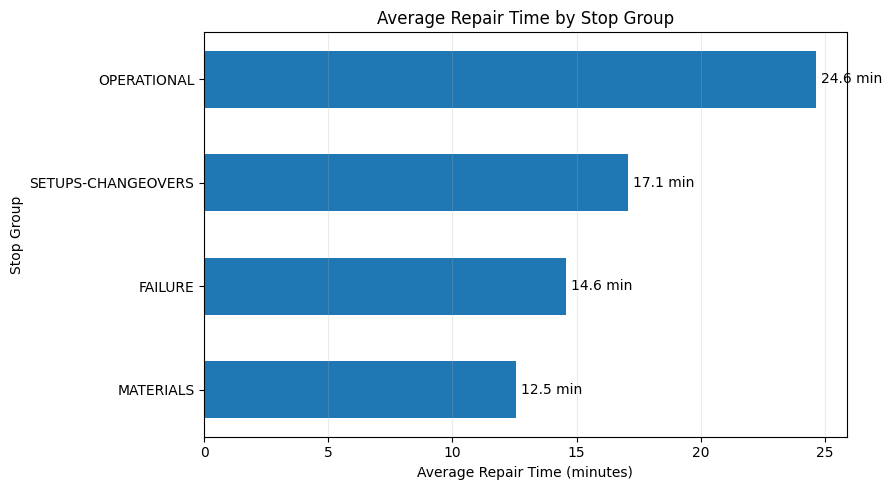
\includegraphics[width=\linewidth]{figures/avg_repair_stopgroup.png}
        \caption{Average Time by Stop Group}
        \label{fig:avg_stopgroup}
    \end{minipage}\hfill
    \begin{minipage}{0.48\textwidth}
        \centering
        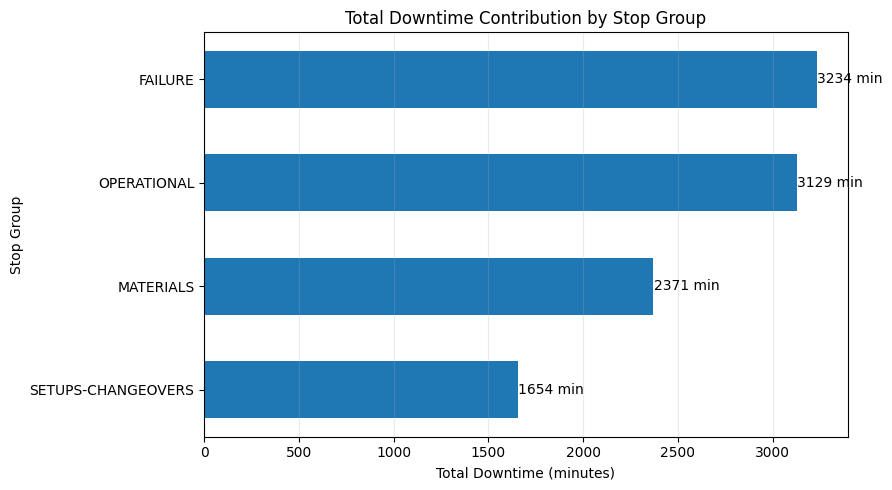
\includegraphics[width=\linewidth]{figures/total_downtime_stopgroup.png}
        \caption{Total Downtime Contribution}
        \label{fig:total_stopgroup}
    \end{minipage}
\end{figure}

\textbf{Engineering Recommendation:}
The plant requires a two-pronged operational strategy to decouple these issues:
\begin{itemize}
    \item \textbf{Operator Empowerment (Operational Delays):} An operational jam should not require a 24-minute response. Line operators (rather than specialized mechanics) should receive upgraded training to safely clear standard operational faults independently. This will drastically reduce the mean time to repair for the \texttt{OPERATIONAL} category.
    \item \textbf{Failure Mitigation (Mechanical Delays):} To reduce the high cumulative downtime from mechanical failures, the focus must shift to component reliability engineering to extend the Mean Time Between Failures (MTBF).
\end{itemize}

\subsubsection*{3. Audit the Afternoon Shift Productivity}

\textbf{Statistical Finding:}\\
There is a statistically significant discrepancy ($p = 0.0051$) in repair efficiency based on the time of day. While the morning shift handles more breakdowns (387 repairs), they resolve them much faster (14.45 min average). The afternoon shift handles fewer overall breakdowns (248 repairs) but takes significantly longer to fix them (19.34 min average).

\textbf{Engineering Recommendation:}
This nearly 5-minute delay per repair is indicative of human or resource constraints rather than mechanical complexity. The plant manager must audit the afternoon shift operations.
\begin{itemize}
    \item Evaluate whether the afternoon shift is chronically understaffed in the maintenance department.
    \item Ensure that senior, highly experienced technicians are distributed evenly across both shifts.
    \item Verify that the parts warehouse and tool rooms remain fully accessible and staffed during afternoon operating hours.
\end{itemize}

\subsubsection*{4. Overhaul the Lean Six Sigma (LSS) Framework and Crisis Protocols}

\textbf{Statistical Finding:}
Our earlier hypothesis tests (Questions 13 and 15) demonstrated that the current Lean Six Sigma implementation failed to statistically reduce the mean repair time. Furthermore, the variability remains dangerously high. The top 10\% of repairs (the 90th percentile) take longer than 31.80 minutes, with catastrophic outliers stretching up to 276.80 minutes (over 4.5 hours). 

\textbf{Engineering Recommendation:}
The generalized LSS rollout is proving ineffective for extreme downtime events.
\begin{itemize}
    \item \textbf{Crisis Protocol Implementation:} The extreme outliers indicate that there is no standardized escalation protocol. The plant should institute a strict "30-Minute Rule": if a machine is not back online within 30 minutes, the issue must automatically trigger an all-hands escalation to the lead engineer or plant manager, preventing standard repairs from ballooning into multi-hour catastrophes.
    \item \textbf{Targeted Root Cause Analysis (RCA):} The LSS team should pivot away from optimizing minor setups and focus exclusively on conducting RCAs for repairs falling in the 90th percentile. 
    \item \textbf{Data Enrichment:} To better predict future downtimes (as explored in Question 19), the plant's MES data collection must be upgraded. The plant must begin logging \textit{technician experience level}, \textit{exact failure severity}, and \textit{machine age}, as our models indicate these latent variables are likely driving the unexplained variance in repair durations.
\end{itemize}